
\chapter{Block Re-Uploading}

\section{Data Re-Uploading}

\cite{P_rez_Salinas_2020} introduced the \textit{re-uploading} encoding technique,
drawing inspiration from classical neural networks.
The key idea that inspired Salinas et al is that a feed-forward neural network processes data several times
(in each layer), one for each neuron in the considered hidden layer. 
Therefore, strictly speaking, data is \textit{re-uploaded} multiple times onto the neural network.
This key concept is illustrated in figure~\ref{Fig:schemes}.


% \subcaption[⟨list entry⟩]{⟨heading⟩}[⟨width⟩][⟨inner-pos⟩]{⟨contents⟩}
% list entry: nome interno che verrà usato se generata la lista delle figure.
% heading: subcaption
% width: larghezza del parbox creato
% inner-pos: posizione che avrà l'immagine nel parbox
% contents: immagine
\begin{figure}
    \centering
    \subcaptionbox[A]{Neural Network}[.4\textwidth][c]{
        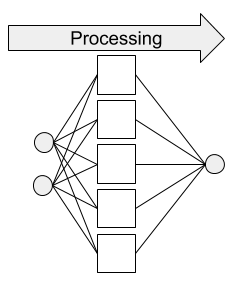
\includegraphics[width=0.25\textwidth]{sections/chapters/Chapter6/Images/Neural_network.png}
        }
    \subcaptionbox[B]{Quantum circuit with re-uploading}[.4\textwidth][c]{
        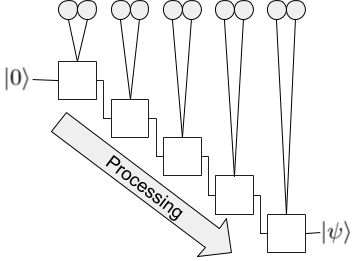
\includegraphics[width=0.5\textwidth]{sections/chapters/Chapter6/Images/Quantum_scheme.png}
        }
    \caption{
        Schemes of a one layer neural network and a single-qubit quantum circuit with data re-uploading.
        In the neural network the data is uploaded in each neuron of the hidden layer, hence data is 
        \textit{re-uploaded} multiple times.
        In a similar way the data is introduced classically numerous times in the circuit.
        The key difference between the two architectures is that each neuron of a neural network processes the 
        data in parallel and simultaneously, whereas the single-qubit quantum circuit with data re-uploading 
        processes the data sequentially.}
\label{Fig:schemes}
\end{figure}

In a single-qubit quantum circuit with data re-uploading, data is introduced as a rotation of the qubit.
Since every unitary can be expressed as the product of three rotation gates, we can define the angles as a linear
combination of weights and coordinates of the data\footnote[1]{Just like in a neuron of neural network.}.

\begin{equation}
    U(\bm{\phi}) = R_Z(\phi_1) R_Y(\phi_2) R_Z(\phi_3)
\end{equation}

For instance, if data is 3-dimensional $\bm{x} = (x_1, x_2, x_3)$:

\begin{align}
    \phi_1 &= x_1 \cdot w_1 + b_1 \\
    \phi_2 &= x_2 \cdot w_2 + b_2 \\
    \phi_3 &= x_3 \cdot w_3 + b_3 \\
\end{align}

If data has a dimension greater than 3, we will need more than one unitary to encode a datapoint.
In general, if data has dimension \textit{d} we will need \(\left\lfloor \frac{d}{3} \right\rceil\) unitaries.
Each repetition of this \(\left\lfloor \frac{d}{3} \right\rceil\) unitaries to encode the data constitutes 
one layer of the architectures.

\begin{figure}
    \centering
    \begin{quantikz}
        \lstick{$\ket{0}$} &&& \gate{U(\phi_1, x)} 
        \gategroup[1,steps=1, style={dashed,rounded corners,fill=blue!20,inner xsep=6pt}, background, label style={label
        position=below, yshift=-0.4cm}]{L(1)} 
        &&& \ \ldots \ &&& \gate{U(\phi_N, x)} 
        \gategroup[1,steps=1, style={dashed,rounded corners,fill=blue!20,inner xsep=6pt}, background, label style={label
        position=below, yshift=-0.4cm}]{L(N)}
        &&& \meter{}
    \end{quantikz}
    \caption{The quantum circuit is divided into layers L(i), which constitutes the building blocks of this 
    architecture.}
\end{figure}


\section{Trainability}

